\documentclass{standalone}

\usepackage{tikz}
\usetikzlibrary{shapes.geometric, arrows}

\tikzstyle{class} = [ellipse, minimum width=4.5cm, minimum height=1cm,text centered, draw=black, fill=yellow!30]
\tikzstyle{input} = [trapezium, trapezium left angle=70, trapezium right angle=110, minimum width=5cm, minimum height=2cm, text centered, draw=black, fill=blue!30]
\tikzstyle{output} = [trapezium, trapezium left angle=70, trapezium right angle=110, minimum width=5cm, minimum height=2cm, text centered, draw=black, fill=green!30]
\tikzstyle{method} = [rectangle, minimum width=5cm, minimum height=2cm, text centered, draw=black, fill=orange!30]
\tikzstyle{base} = [rectangle, rounded corners, minimum width=2cm, minimum height=2cm,text centered, draw=black, fill=red!30]
\tikzstyle{cond} = [diamond, minimum width=5cm, minimum height=2cm, text centered, draw=black, fill=white!30]

\tikzstyle{arrow} = [thick,->,>=stealth]

\begin{document}
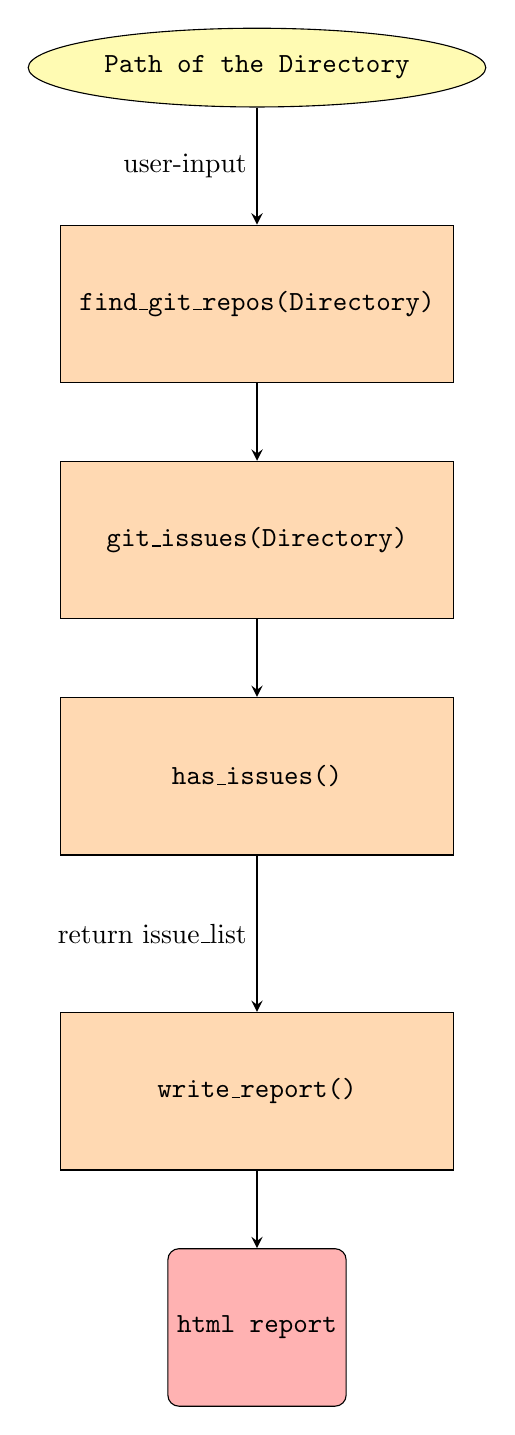
\begin{tikzpicture}[node distance=2cm]

% objects
\node (class) at (0,0) [class] {\texttt{Path of the Directory}};
\node (method1) at (0,-3) [method] {\texttt{find\_git\_repos(Directory)}};

\node (method2) at (0,-6) [method] {\texttt{git\_issues(Directory)}};

\node (method3) at (0,-9) [method] {\texttt{has\_issues()}};
\node (method4) at (0,-13) [method] {\texttt{write\_report()}};


% \node (method4) at (8,-13) [method] {\texttt{incPos(temp, pos, size)}};
\node (base) at (0,-16) [base] {\texttt{html report}};


% arrows
%\draw [arrow] (class) -- (method1);
\draw [arrow] (class) -- node[anchor=east] {user-input} (method1);
\draw [arrow] (method1) -- (method2);
\draw [arrow] (method2) -- (method3);
\draw [arrow] (method3) -- node[anchor=east] {return issue\_list} (method4);
\draw [arrow] (method4) -- (base);



\end{tikzpicture}
\end{document}
